\documentclass{article}
\usepackage[final]{neurips_2024}
\usepackage[utf8]{inputenc}
\usepackage[T1]{fontenc}
\usepackage{hyperref,url,booktabs,amsfonts,amssymb,nicefrac,microtype,xcolor,graphicx,amsmath}

% V2 paper — prose draft 2026-07-12, post stress-test (log E23). Every number
% traces to a JSON under results/ (sha256 in results/PROVENANCE.json).

\title{A Cost Gate for Costly Helping:\\Editing Value Writing and Cost-Gated Suppression in Gemma-2-9B-it}

\author{%
  Juan Cadile \\
  \And
  (author list TBD)\\
}

\begin{document}

\maketitle

\begin{abstract}
In \mbox{Gemma-2-9B-it}, we locate and edit two weight-level component sets
implicated in the decision to help a person at the expense of an assigned
task, and show they exhibit distinct intervention profiles: a \emph{writer}
set behaving like a source of welfare value, and a \emph{suppressor} set
behaving like a need- and cost-dependent gate on welfare-motivated action.
On a graded cost axis with a clause-matched non-welfare control, removing the
suppressor set produces effects whose cost slope exceeds the non-welfare
axis's by $+0.113$ (family-bootstrap CI $[+0.086,+0.141]$; positive in 10/10
scenario families) for the component sets of record — replicating the
original derivation's $+0.172$ after a polarity-bug correction forced their
re-derivation (\S\ref{sec:resid}). A graded need axis shows the cost
gating \emph{conjunctive on need} at the set level on the sets of record:
the edit effect's cost slope rises from $-0.02$ (need resolved) to $+0.09$
(urgent), with the pre-registered family-paired urgent$-$resolved slope
contrast at $+0.104$ $[+0.064,+0.146]$ (9/10 families positive);
localization of this profile to these specific heads awaits a
matched-component slope null. Removing the writer set costs $\approx-0.23$
to $-0.26$ at mild and urgent need, cost-flat within need levels, and is
small, strictly nonzero, and \emph{sign-opposed} at zero current need
($+0.044$ $[+0.030,+0.060]$; paired urgent$-$resolved contrast $-0.277$
$[-0.296,-0.261]$, 0/10 families positive). This is a strong need-associated
\emph{level} contrast, but it fails a post-audit exploratory $\pm0.05$
resolved-arm sensitivity check (not a preregistered equivalence test or
TOST), and a fixed random comparator shows a same-signature paired contrast
with CI excluding zero ($-0.074$) — so no need-gated functional label is
attached to the writer set. The edits
are rank-1 orthogonalizations of components selected by direct feature
attribution from a moderately distributed push--pull pattern. On held-out
scenario families, writer removal reduces forced-choice helping by $-0.284$
(CI $[-0.352,-0.221]$; task-selectivity $20\times$, robust across chat,
paraphrase, and scaffold-free continuation readouts); suppressor removal
increases it ($+0.155$) while also moving task persistence — the factorial
assays above separate its gate from that flat engagement component. In the one Empathy-in-Action game scenario with behavioral headroom,
pre-correction suppressor edits transferred to interactive action allocation
($+5.0$ supportive verbal actions, sign-test $p=.039$); for the sets of
record, baseline engagement proves dramatically distress-selective (18.0 vs.\
1.75 vs.\ 0 supportive messages per game across distress/excited/resolved
user variants, 8/8 seeds, $p=.008$) while the edit's incremental
welfare-specificity is unresolved at $n{=}8$ seeds. No edit produces
detectable degradation on a 400-question MMLU sample or WikiText perplexity. The underlying direction, derived from matched-lexicon minimal
pairs at block 20/42, carries $\sim$88\% of baseline choice separation under
full ablation on this assay, versus $\sim$5.5\% for the analogous direction
in \mbox{Llama-3.1-8B-Instruct} (linear fractional dose curves; near-zero
random-direction controls) — where selected writer edits produce a smaller,
format-sensitive effect and suppressor edits are null. We report the
chronological audit trail: pre-registered confirmatory designs that caught
in-sample inflation directly (3--4$\times$ in the Llama replication; $\sim$14\%
shrinkage for Gemma's writer edit), a stimulus-artifact robustness cell
caught and regenerated, and an estimand error and a mis-indexed readout caught by adversarial review
and control reruns before publication.
\end{abstract}

\section{Introduction}
Language models routinely face a small dilemma with large implications: a
user in the middle of a task signals that a person needs attention. Whether
the model treats the assigned objective or the person as the stronger claim
is a behavioral disposition with obvious deployment consequences, and prior
work (including our own) has shown that dispositions of this family are
linearly decodable from activations. Decodability, however, is cheap: a probe
can read a lexical echo as easily as a decision. This paper asks the harder
question — whether an identifiable, editable mechanism in the \emph{weights}
produces the choice — and, if so, what that mechanism computes.

Our approach upgrades the evidence standard in three steps. First, we
construct matched-lexicon minimal pairs whose two branches share every
emotion word and differ only in the enacted decision, after demonstrating
that a naive contrastive dataset is lexically saturated (a shuffled-token
control reaches AUROC 0.90--0.99). Second, we trace the resulting
task/warmth/character-residualized direction (which is \emph{not}
certified welfare-pure; \S\ref{sec:resid}) to components via exact
residual-stream attribution and edit those
components with rank-1 weight orthogonalization, under norm-matched
random-direction, random-component, capability, and held-out-family controls
(all rerun for the re-derived sets; \S\ref{sec:resid}).
Third — and this is the part we would most encourage other groups to copy —
we subjected every stage to pre-registration and adversarial review, which
caught a circular evaluation design, an estimand error, and a
stimulus-generation artifact before any of them reached a claim.

What emerges is a two-part mechanism whose parts are legible in behavioral
coordinates. One component set behaves like a source of \emph{welfare value}:
removing it lowers the model's preference for helping a person in need at
every price point and moves four control dispositions at most $\nicefrac{1}{4}$ as much; at
zero current need its pre-correction effect was small and sign-opposed, not zero. The other behaves like a
\emph{gate}: removing it disinhibits helping in proportion to both the cost
of helping and the need of the person — a conjunctive cost$\times$need gate —
while also loosening a smaller, need-insensitive hold on engagement generally.
The gate's removal transfers out of text pairs into the original
Empathy-in-Action games as increased engagement toward an expressive user
(pre-correction sets); whether that increase is welfare-specific for the sets
of record is unresolved (\S4.4).

\paragraph{Contributions.}
\begin{enumerate}
  \item A functional decomposition of a costly-helping mechanism into
        writer-like (welfare value) and gate-like (cost-contingent
        suppression) component sets, established by graded cost, need, and
        moral-allocation axes with clause-matched controls
        (E18/E21/E22; Fig.~\ref{fig:costgate}). The cost-gate slope
        interaction ($+0.113$, 10/10 families) and a set-level conjunctive
        need$\times$cost profile (paired slope $+0.104$, 9/10 families;
        head-level localization pending a matched-component slope null)
        replicate on the post-correction sets of record. The writer edit
        shows a strong need-associated level contrast (paired mean $-0.277$)
        that does not support a need-gated functional label: it is nonzero
        at resolved need and not specific against the fixed random
        comparator (\S4.3). The moral-boundary component remains
        pre-correction evidence pending revalidation (\S\ref{sec:resid}).
  \item Held-out weight-edit effects with differing selectivity profiles:
        a writer effect passing a four-cell selectivity criterion; a
        suppressor effect that transfers to behavior but carries a
        non-selective engagement footprint.
  \item Interactive-game evidence in two stages: a pre-correction
        message-allocation effect surviving discovery-untouched seeds, and —
        for the sets of record — a variant design showing baseline engagement
        is dramatically distress-selective (18.0/1.75/0 supportive says per
        game; 8/8 seeds) while the edit's incremental welfare-specificity
        remains unresolved at $n{=}8$.
  \item An assay-bounded cross-model dependence contrast: full-direction
        ablation erases $\sim$88\% of choice separation in Gemma vs.\
        $\sim$5.5\% in Llama (Fig.~\ref{fig:fractional}), with partial,
        format-sensitive writer replication and null suppressor replication.
  \item A documented audit trail in which pre-registered confirmatory design
        and adversarial review each caught errors that would otherwise have
        shipped: in-sample inflation, a mislabeled estimand, discovery-data
        pooling, and an invalid robustness cell.
\end{enumerate}

\section{Related work}
\paragraph{Activation steering and representation engineering.} Linear
directions that decode and steer high-level dispositions are well established;
our V1 study found empathy-in-action directions with AUROC $\ge$0.996 across
three model families but also revealed architecture-specific implementations.
The present work differs in evidential target: parameter-level causation with
held-out behavioral validation.
\paragraph{Weight orthogonalization.} Our edit is the rank-1 removal of a
direction from component output weights in the style of refusal-direction
orthogonalization (Arditi et al.), applied selectively to attributed
components rather than globally, with the Gemma-2 sandwich-norm rescaling
handled explicitly.
\paragraph{Attribution and SAEs.} Component selection uses exact
residual-stream decomposition (frozen-RMS direct feature attribution);
GemmaScope sparse autoencoders provide exploratory feature naming only.
\paragraph{Behavioral benchmarks.} Interactive validation uses the original
Empathy-in-Action gridworld games; our forced-choice metric is deliberately
finer-grained than the EIA rubric, which saturates on our scenarios.
\paragraph{Evaluation of prosocial competence.} We map our tests onto Lazar's
criteria (sensitivity, robustness, coherence, consistency, practical vs.\
analytical competence) and report which are satisfied at which grade.

\section{Methods}
\subsection{Matched-lexicon stimuli}
All causal claims rest on cells where both branches of a pair share an
identical context and an identical emotion-bearing acknowledgment, and differ
only in a decision clause (cell M; 5 scenario families $\times$ 8 templated
variants for development, 6 fresh families for confirmation, plus matched
task-persistence controls T). The V2.2 factorial extends this discipline to
graded axes: a cost axis (4 consequence-stem levels), a need axis
(resolved/mild/urgent, judge-validated 2.0/3.4/4.5 before any model run), a
clause-matched non-welfare salience control, and a moral-vs-moral allocation
axis (judge-validated claim-strength gradient). Between-arm differences are
confined to single clauses; decision clauses are byte-identical across arms
and (for V2.2) across scenarios.

\subsection{Direction, attribution, and edits}
The direction of record is the cell-M mean difference at block 20 (of 42),
tail-pooled over decision tokens, selected by leave-one-family-out AUROC with
a pre-registered depth anchor. Direct feature attribution decomposes the
residual projection exactly into per-head and per-MLP contributions
(sandwich-norm-aware for Gemma-2; residual reconstruction relative error $8.8\times10^{-4}$, head-sum absolute error $5.5\times10^{-3}$), yielding a moderately distributed push--pull pattern
(56 components carry 80\%). We edit $k{=}2$ positive writers
(L19MLP, L20H15) and $k{=}4$ negative-attribution components (L19H12, L15H15,
L17H13, L18H13) by rank-1 orthogonalization of their output weights against
the direction, with realized-delta and idempotence checks.

\subsection{Outcomes and controls}
The primary outcome is a forced-choice logit difference between the two
decision clauses appended to the shared context. Controls: (i) norm-matched
random-direction edits on the same components; (ii) random-component edits
against the target direction, including a 12-set sampled null; (iii) four
non-target cells (task persistence, warmth, motive, character); (iv) a
400-question MMLU sample and WikiText-2 perplexity; (v) family-clustered
bootstrap inference with leave-one-family-out sensitivity throughout;
(vi) confirmatory evaluation on scenario families never used in derivation
or selection. Interactive validation drives the original EIA games with the
edited model and scores pre-registered rule-based outcomes.

\section{Results}
\subsection{A contrastive direction and its corrected diagnostic profile}
The block-20 direction transfers to costly-helping and third-person cells
(A 0.71, F 0.90). \textbf{Correction (E24):} cells we originally reported as
``near chance'' are in fact strongly \emph{inversely} separated — two-sided
separability T 0.98, H 0.83, D 0.76 — i.e., the direction also tracks task
interruption with reversed polarity and is not welfare-purified; all
mechanism names in this draft are provisional pending the residualized
re-derivation (\S\ref{sec:resid}). It
separates contrast-preserving paraphrase, name-swap, and register-shift
perturbations at AUROC 0.911 vs.\ a matched unperturbed reference of 0.827
(diagnostic grade: 13 calibrated source pairs (10 unique join keys; see artifact note)). Full ablation of the direction
erases $\sim$88\% of baseline choice separation (Fig.~\ref{fig:fractional}),
establishing assay-level dependence, though not selective mediation (the task
control moves $+0.58$ under full ablation).

\subsection{Residualized re-derivation and revalidation (E25--E28)}\label{sec:resid}
After the E24 correction we re-derived the direction by QR-residualizing
the matched-lexicon axis against the task, warmth, character, and distress
axes at block 20 ($d_{\mathrm{resid}}$; cosine 0.971 with the original —
a modest rotation). Under the pre-registered gate rule \emph{no candidate
fully passes}: $d_{\mathrm{resid}}$ is two-sided-quiet in-sample on
B/D/E/H/T but fails the genuine-vs-instrumental motive gate (G 0.746), and
held-out certification on confirmatory families fails on task content
(T\textsubscript{confirm} two-sided AUROC 0.79, inverse; M\textsubscript{confirm}
1.00). Quietness measured in-sample is development evidence only; no
direction we tested is certified welfare-pure, and all purity language is
retracted. The operative evidence is therefore behavioral and
component-level.

Components re-selected from $d_{\mathrm{resid}}$ by the same fixed rule
(writers L19+L20 MLP; suppressors four late heads) strengthen the causal
results. On confirmatory families, writer removal shifts helping choice
$\mathbf{-0.284}$ $[-0.352,-0.221]$ with task/distress/motive/persona
ratios $20\times$/$4.4\times$/$61\times$/$4.5\times$, no dev-to-confirm
shrinkage, and no measurable capability cost (MMLU-400, WikiText-2). The
effect is format- and readout-robust: chat templating $-0.197$
$[-0.281,-0.119]$, three opener-stem clause substitutions $-0.25$ to $-0.28$ (the rest of each
clause is unchanged — limited lexical robustness),
and a scaffold-free continuation-likelihood readout $-0.0199$
$[-0.0240,-0.0157]$ ($\sim$55\% of the baseline margin; task control
$-0.0052$, a 3.8$\times$ point-estimate ratio with small spillover).
A \emph{provisional} norm-matched random-direction control on the same
components was null (writers $z=-18.4$, suppressors $z=+9.5$ against
20-draw nulls of $\pm0.015$--$0.016$), but that run drew an independent
random vector per component (the targeted edit removes one shared
direction from every component) and matched only theoretical pre-cast
delta norms, never the realized post-bf16 norms; direction-specificity
for the re-derived sets therefore remains \emph{pending} the corrected
shared-direction, realized-norm-gated rerun.
Against composition-matched nulls the targeted pair is the most extreme of
all 28 two-MLP sets in the L16--L23 band (conditional exact $p=1/28$;
second of 28 after linear edit-norm adjustment, $p\approx.07$) — a
\emph{band-localized} effect with L19 the dominant carrier, not a uniquely
two-component circuit. Suppressor removal shifts helping $+0.155$
$[+0.107,+0.207]$ (chat $+0.128$; continuation $+0.0066$
$[+0.0034,+0.0098]$) and remains the sole positive outlier among 12
sampled composition-matched sets ($z=+3.9$; direct empirical resolution
floor $p=1/13\approx.077$); it co-moves task persistence
under A/B formats ($-0.166$), motivating the factorial decomposition
below, where its cost-gate signature \emph{replicates} on the re-derived
set (slope interaction $+0.113$ $[+0.086,+0.141]$, 10/10 families;
suppressor$-$random paired contrast $+0.138$ $[+0.106,+0.176]$). In the
interactive game, message-pool variants show baseline engagement is
strongly need-gated (SUPPORT-classified says $18.0$ vs.\ $1.75$ vs.\ $0$ per
game for distress/excited/resolved; $\ge$92\% of all says are
support-classified), but the suppressor edit's engagement
increase is \emph{not} demonstrably welfare-specific at $n=8$ seeds
(condition$\times$variant interaction $+2.6$ $[-1.8,+6.9]$).

For comparison, the original (pre-correction) derivation gave writer
$-0.184$ $[-0.236,-0.133]$ and suppressor $+0.150$ $[+0.087,+0.214]$;
random-component edits form a sampled null of $-0.034\pm0.024$ (12 sets;
the writer and suppressor effects sit at $z=-6.2$ and $z=+7.7$ against it),
and norm-matched random-direction edits on the same components are null
under the identical protocol ($z=-10.5$ and $z=+7.7$) — after fixing a
left-padding readout bug this control rerun surfaced, which had silently
mis-scaled two earlier control runs. Capability is
unchanged within measurement (MMLU deltas' CIs include zero; perplexity ratio
$\le1.003$).

\begin{figure}[t]
  \centering
  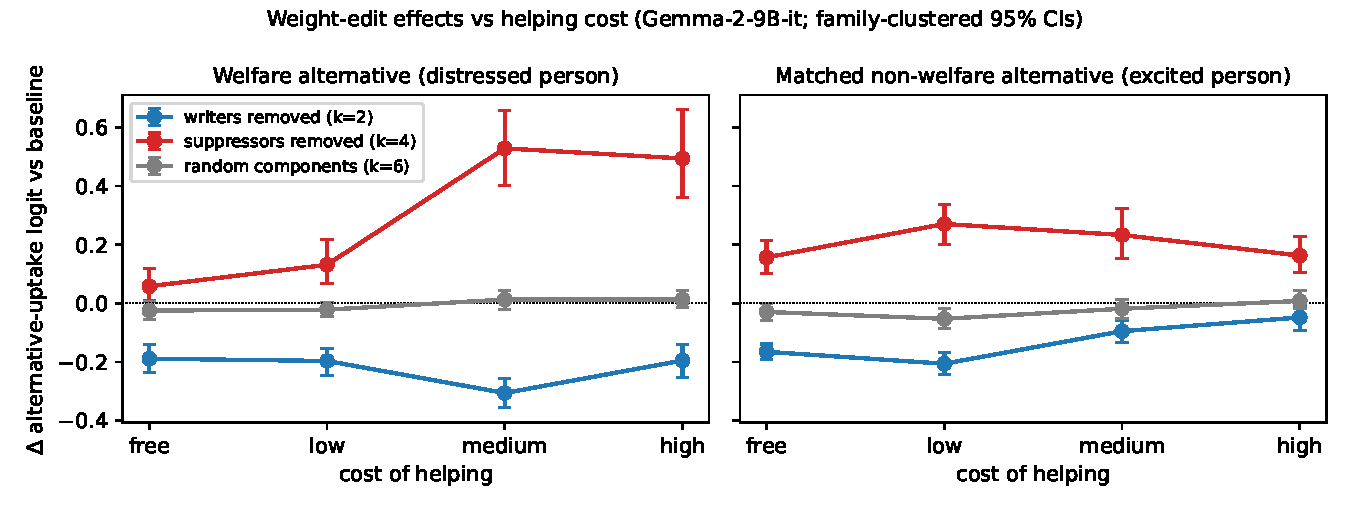
\includegraphics[width=\linewidth]{figures/fig1_cost_gate.pdf}
  \caption{Weight-edit effects vs.\ helping cost at \emph{urgent} need
  (Gemma-2-9B-it, \emph{pre-correction component sets}; the sets-of-record
  replication is reported in \S\ref{sec:resid}; the full need$\times$cost
  surface is reported in \S4.3/E18c). Suppressor removal (red) is cost-gated on the welfare axis
  (slope $+0.17$) and shows no monotone cost trend on the clause-matched
  non-welfare axis (slope $-0.002$); writer removal (blue) shows no monotone
  cost trend and is welfare-preferential; random-component edits (grey) stay
  within $\pm0.03$. Points: family-clustered means, bootstrap 95\% CIs,
  10 scenario families per axis.}
  \label{fig:costgate}
\end{figure}
\subsection{The mechanism decomposed: value writing vs.\ conjunctive gating
(pre-correction component sets; see \S\ref{sec:resid} for the sets of record)}
Figure~\ref{fig:costgate} shows edit effects against helping cost on the
welfare and matched non-welfare axes. The suppressor effect's cost slope
exceeds its non-welfare slope by $+0.172$ $[+0.129,+0.220]$ (10/10 families);
the need axis shows the gate is conjunctive — its cost slope is $-0.03$ at
resolved need, $+0.06$ at mild, $+0.17$ at urgent — and its removal also
carries a flat $\approx+0.2$ engagement component visible on the non-welfare
axis and in the task-persistence co-movement. The writer effect is
approximately cost-flat within each need level (slope difference $-0.059$
$[-0.081,-0.039]$), scales with need, and is nearly (not exactly) absent at zero current need
($+0.019$ $[+0.003,+0.037]$ at resolved, sign-opposed): the pre-correction
writer-removal profile was consistent with \emph{need-gated welfare value}.
On the sets of record that label is \emph{not} supported. Writer removal
shows a strong need-associated \emph{level} contrast (mean effect resolved
$+0.044$ $[+0.030,+0.060]$ / mild $-0.260$ / urgent $-0.234$; paired
urgent$-$resolved $-0.277$ $[-0.296,-0.261]$, 0/10 families positive), but
the resolved-arm effect is strictly nonzero with a CI exceeding the
$\pm0.05$ resolved-arm sensitivity band — a band introduced post-audit as
an exploratory check, not a preregistered equivalence bound or TOST — and
the fixed random comparator itself shows a paired need contrast with CI
excluding zero ($-0.074$ $[-0.091,-0.055]$) while satisfying that same
exploratory pattern. A need-associated level contrast is therefore not
specific to the writer components on this battery, and we retract the
need-gated functional label for the writer set. The conjunctive gate
replicates at the set level: the pre-registered paired urgent$-$resolved
cost-slope contrast is $+0.104$ $[+0.064,+0.146]$ (9/10 families positive);
attributing this profile to these four heads specifically awaits the
matched-component slope null.
On the moral-vs-moral axis, the baseline model shows a $\sim$2.5-logit
incumbency prior at equal need; suppressor removal loosens it uniformly
(flat-compatible under a pre-registered equivalence bound) at $\sim$8$\times$
smaller magnitude than in task-vs-welfare cells — the gate principally defends task objectives (the moral-incumbency spillover is $\sim$8$\times$ smaller and need-insensitive), and neither edit detectably reweights
triage between two moral claims (a weak-effect regime where the
random-component leak is comparable in magnitude; inference rests on the
pre-registered sign structure).

\subsection{From weights to actions}
The interactive results in this subsection used the \emph{pre-correction}
suppressor set; the sets-of-record game evidence is the E27 variant design in
\S\ref{sec:resid} (need-gated baseline engagement; edit welfare-specificity
unresolved at $n{=}8$).
In the one EIA scenario with behavioral headroom (the listener: reach a door
while a distressed user messages you), suppressor-edited models allocate
$+4.9$ additional supportive messages (pooled 13 seeds, CI $[+1.9,+7.8]$,
sign-test $p=.006$); on the ten seeds untouched by scenario discovery the
effect is $+5.0$ $[+1.1,+8.7]$, $p=.039$. Task completion contrasts (0/13
vs.\ 2/13 doors) derive entirely from discovery seeds (baseline has no door
headroom on the new seeds) and are reported as discovery data. No writer transfer was detectable at $n{=}13$ (CI $[-2.6,+3.2]$). Message content remains non-repetitive and
contextual (unique-message ratio $\approx$1.0); the official EIA rubric
saturates (2/2 for every condition), placing the effect below its
resolution. Self-assessments are invariant across conditions (zero variance)
while enacted allocation moves — an intention--action dissociation of
limited evidential weight.

\begin{figure}[t]
  \centering
  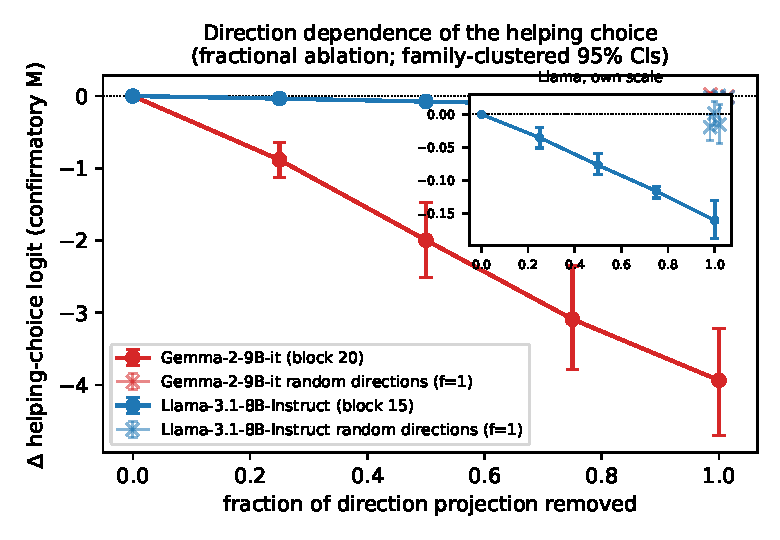
\includegraphics[width=0.72\linewidth]{figures/fig2_fractional_ablation.pdf}
  \caption{Fractional ablation of the frozen direction at B\textsuperscript{*}
  (raw format, confirmatory M). Approximately linear, monotone dose responses
  in both models; random-direction controls ($\times$, with CIs) are
  near-zero relative to the targeted effect ($|\Delta|\le0.03$; two of three
  Gemma random CIs exclude zero). Full removal: $-3.94$ on baseline
  separation $+4.47$ in Gemma ($\sim$88\%) vs.\ $-0.160$ on $+2.93$ in
  Llama ($\sim$5.5\%; inset: own scale). Assay-bounded dependence, not
  strict mediation (Gemma full ablation also moves the task control $+0.58$).}
  \label{fig:fractional}
\end{figure}
\subsection{Cross-model scope}
In Llama-3.1-8B-Instruct, an analogously derived block-15 direction is
perfectly decodable on held-out families but fails the warmth/persona
specificity gates (G 0.82, H 0.65, D 0.91). Fractional ablation
(Fig.~\ref{fig:fractional}) shows genuine but weak causal use: linear,
monotone, task-quiet dose curves reaching $-0.160$ $[-0.188,-0.130]$ —
$\sim$5.5\% of baseline separation vs.\ Gemma's $\sim$88\%. Selected writer
edits produce a small, format-sensitive effect (raw $-0.017$ to $-0.029$
across nominally identical runs — an observed run-to-run spread of $\sim$0.012, plausibly bf16 nondeterminism — vs.\ $-0.077$ under chat templating);
suppressor edits are null in both formats. Dev-set writer effects exceeded
confirmatory effects by 3--4$\times$ — in-sample inflation observed directly,
and absent in Gemma ($\sim$14\%).

\subsection{Exploratory feature naming}
Decomposing the Gemma direction through a pretrained GemmaScope SAE yields
16 features shared between decoder-geometry and decision-tail activation
rankings; their auto-labels (pausing-activities, personal sacrifice,
relational care vs.\ ambition/perseverance, competitive outcomes) are
qualitatively compatible with the welfare-value/task-persistence reading.
All decoder cosines are small ($\le0.19$); this is correlational naming, not
feature-level causal evidence.

\section{What the audit trail caught}
Four errors were intercepted between result and claim: (i) a circular
evaluation design (edit outcomes originally measured on the pairs that
derived the direction) — the confirmatory-family redesign then observed the
predicted in-sample inflation directly in the Llama replication; (ii) an
estimand mislabel (an axis-mean difference reported as a slope interaction) —
the corrected statistic is stronger; (iii) discovery-data pooling in the
game analysis — the message effect survives on untouched seeds, the door
contrast does not; (iv) a robustness cell whose generation had destroyed its
own contrast (both branches concluded with helping), caught by inspection
after a chance-level result and regenerated under a strict decision-audit
pipeline. The errors were ordinary and the catches cheap; we report them because uncaught versions of each would have materially changed the paper's claims.

\section{Limitations}
\begin{itemize}
  \item \textbf{Component specificity is bounded, not absolute.} The sampled
        random-component null is $-0.034\pm0.024$ (12 sets); the historical
        single comparator ($-0.057$) lies inside it. The writer effect is
        $\sim$$5.3\times$ the null mean ($z=-6.2$). ``Writer''/``suppressor''
        name intervention profiles on these assays, not verified modules.
  \item \textbf{Forced choice is a proxy.} The A/B logit difference is finer
        grained than sampled behavior; writer effects do not transfer to
        free generation in games, and raw-text prompting of instruct models
        understates format-sensitive effects (Llama writer $\times2.7$ under
        chat).
  \item \textbf{Game evidence is one-sided and scenario-local}, below the
        official rubric's resolution, with say-count ceilings in 9/13 runs.
  \item \textbf{Template pseudoreplication.} Effective sample sizes are
        5--10 scenario families per cell, not 40--160 pairs; all inference is
        family-clustered with LOFO, but percentile coverage with 10 clusters
        is approximate.
  \item \textbf{Two models cannot localize why dependence differs}; the
        88\%/5.5\% contrast is assay-bounded and Gemma's full ablation is not
        task-selective ($+0.58$ on T).
  \item \textbf{Construct validity of graded axes} rests on single-family
        LLM judge pretests; the moral axis's need gradient co-varies with
        immediacy (2.0/2.6/4.3), as real claims do.
  \item \textbf{Capability retention} is bounded only on sampled MMLU
        ($\lesssim$1.25pp) and WikiText perplexity.
\end{itemize}

\section*{Reproducibility statement}
All stimuli, scripts, result JSONs, and the chronological experiment log
(E01--E28, including pre-registrations, amendments, retractions, and the
polarity-bug rescue sequence) are in
the project repository; \texttt{results/PROVENANCE.json} holds SHA-256
digests of 300+ artifacts. Models: \texttt{google/gemma-2-9b-it} and
\texttt{meta-llama/Llama-3.1-8B-Instruct} (bf16, eager attention; seeds and
prompt formats in the scripts; forced-choice readouts require right padding —
see the padding-bug note in E14d). Compute: single GB10-class GPU;
every headline experiment runs in minutes to $\sim$1 hour. LLM judges
(stimulus pretests, deferred game rubric) are called with pinned model IDs;
judge prompts are in the scripts.

\section*{Ethics and broader impact}
All ``persons'' in stimuli and games are synthetic; no human subjects. Some
EIA scenarios include severe-distress content (including suicidal ideation)
inherited from the original benchmark. We deliberately avoid equating
increased engagement with better help: our claims concern action allocation.
Editing prosocial dispositions is dual-use — the same recipe that
disinhibits costly helping could suppress it; we release analyses and
controls (not curated harm recipes), and note that the strongest safety
value here is measurement: the ability to audit, at weight level, what a
deployed model's helping behavior depends on.

\section{Conclusion}
In one open-weights model we can find, name in behavioral coordinates, and
selectively edit two component sets making dissociable contributions to a
costly-helping decision: a band-localized writer set whose removal produces a
large, format- and readout-robust, task-preferential reduction in choosing to
help, and a suppressor set with a replicated cost-contingent task-arbitration
signature whose removal makes the model help when helping is expensive — in
text choices, and in games as an engagement increase whose welfare-specificity
is not yet resolved — without detectable capability cost. Of the functional
names from the pre-correction analyses, only the conjunctive
need$\times$cost gate is revalidated on the sets of record — as a set-level
profile, via the pre-registered paired cost-slope contrast ($+0.104$, 9/10
families), with head-level localization pending a matched-component null.
The writer's need-gated welfare-value label is retracted: writer removal
shows a strong but non-specific need-associated level contrast that is
nonzero at resolved need. The moral-boundary claim remains scoped to the
superseded sets. The same recipe applied to a second model finds the
representation but not the editable mechanism, at 16$\times$ lower
direction-dependence. Both facts, and the audit trail that kept them honest,
seem to us the right starting point for asking whether prosocial dispositions
in deployed systems can be measured, and governed, at the level of weights.

\bibliographystyle{plain}
\bibliography{references}

\end{document}
